\chapter{电力系统的脆弱性研究}
\label{cha:theory}

\section{引言}
\label{sec:index3}


\section{电力系统脆弱性}
\label{sec:defina}


\subsection{电力系统稳定性、可靠性、鲁棒性的区别与联系}
\label{sec:network}



\subsection{电力系统脆弱性的本质及脆弱过程分析}
\label{sec:network}



\subsection{电力系统脆弱性的数学描述}
\label{sec:network}


\section{电力系统结构脆弱性研究}
\label{sec:powersys}



\subsection{电力系统结构脆弱性定义与数学描述}
\label{sec:network}



\subsection{基于复杂网络的结构脆弱性研究}
\label{sec:network}


\subsection{基于$PageRank$的结构脆弱性研究}
\label{sec:pagerank}
$PageRank$最早是被用来作为互联网网页结构的模型,并且对所有网页的重要度进行量化评估的一种算法\cite{PR1,PR2,PR3}。在众多计算互联网网页的相关性的算法中,$PageRank$是名气最大,且最早被谷歌浏览器采用的。$PageRank$的基本思想是一个网页的重要性依赖于所有链接向它的其他网页。比如,网页$i$有链接指向网页$j$,如果有很多其他网页有链接指向网页$j$,那么我们认为,网页$j$是非常重要的。另一方面,若只有一个网页有链接指向网页$j$,但是这个网页是一个权威性很高的网址,如谷歌,百度等网页,我们认为网页$j$也非常重要,因为由受欢迎、权威的网页指向它,这份重要性将会传递下来。

电网中,每条支路上的潮流是有确定的方向的,所以可以被视为一个有向图。其中,每个母线节点被视为一个网页,母线节点之间的电气连接被视为网页中的超链接,根据电流的方向决定超链接的方向。互联网与电网的$PageRank$的拓扑模型比较如表~\ref{tab:PRComparision}。已有的研究中,大多学者在$PageRank$模型的网页出链的处理上采用均分的思想\cite{PRNET},本文在综合考虑潮流能量对结构的影响下,认为出链是按照实际的潮流的比重进行分配的。

即按照网页的超链接可以传递重要性的思想,假设$A$节点拥有~3~个出链,它会分别按照视在功率的比例分别传递给所指向的$B$、$C$、$D$三个节点,按照能量的分布作为权重。根据重要性传递规则,可以得到能量转移矩阵$A$。对于没有出链的节点,则按照$PageRank$的算法,认为该节点对所有节点都出链,从而解决终止点的问题。因为电网的潮流能量分布中不存在自己指向自己的连接,故不存在陷阱问题,因此不予考虑。
\begin{table}[htb]
  \centering
  \caption{互联网与电网的$PageRank$拓扑模型比较}
  \label{tab:PRComparision}
    \begin{tabular}{C{4.5cm}C{4.5cm}C{4cm}}
      \toprule
      互联网 & 电网 & $PageRank$拓扑 \\
      \midrule
      网页 & 母线 & 节点\\
      超链接 & 输电支路 & 有向边\\
      指向该网页的网页数目 & 母线进线数目 & 入度\\
      该网页指向的网页数目 & 母线出线数目 & 出度\\
      \bottomrule
    \end{tabular}
\end{table}

$PageRank$算法应用于电网拓扑的具体步骤为:

$(1)$假定初始服从均匀分布,即每个母线节点的重要性都是相同的,即对于一个一共有$n$个节点的系统而言,赋予每个网页初始相同的$PR$值,一般都为1。

$(2)$根据电网的实际潮流计算每条连接上的视在功率得到能量分布权重的矩阵P,再根据公式\ref{equ:chap3:Index3}得到能量转移矩阵A。

$(3)$迭代计算,由于每个超链接的存在都会增加对应网页的$PR$值,所以通过考虑潮流连接、能量转移情况对各个母线节点的$PR$值进行迭代更新。

$(4)$最后,经过若干次的迭代后,各个母线节点的$PR$值会趋于一个稳定的值。
\begin{equation}
\label{equ:chap3:Index3}
PR(p_i)=\frac{1-q}{N}+q\sum\limits_{p_j\in\mathbf{M_{p_i}}}{\frac{PR(p_j)}{L(p_j)}}
\end{equation}

式~(\ref{equ:chap3:Index3})中,$p_i$是被计算的节点,$M_{p_i}$是节点$p_i$的入链节点集合,$L(p_j)$是节点$p_j$的出链数目,$N$是节点总数目。$q$为阻尼系数,一般取~0.85~,引入该参数是为了解决出链为零的节点在模型计算中带来的问题,代表了当前的母线节点没有遭到破坏正常运行的概率。$1-q$则代表了节点遭到意外破坏退出运行的概率。从公式中可以看出,$p_i$节点的$PR$值与和它相连的$p_j$节点的$PR$值有关,其值越大,且$p_j$节点的出链越少,$p_i$节点的$PR$值越大。其计算流程图如下:
\begin{figure}[H] % use float package if you want it here
  \centering
  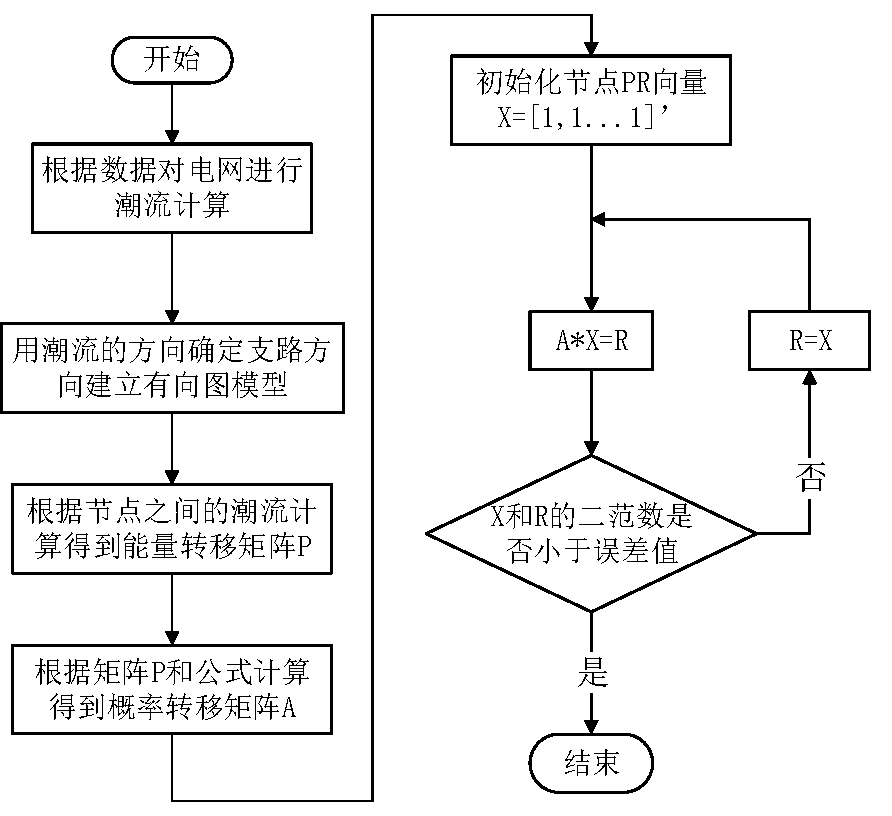
\includegraphics[height=8.4cm]{PRprocess.pdf}
  \caption{$PangRank$计算流程}
  \label{fig:PRPro}
\end{figure}

由图可知在$PageRank$在计算中,考虑更多的是节点的重要性在拓扑中的传递性。即通过反复迭代,确保所有节点的$PageRank$值在整个拓扑的重要性分配中趋于稳定,误差达到最小。$PR$值代表了节点在网络中的重要程度,$PR$值越高,节点越重要。

\subsection{模型比较与案例分析}
基于前面的研究可知,对电力系统的拓扑建模有两种不同的角度。不考虑潮流的方向,关注支路的重要性可将系统视为一个加权无向图。反之,考虑潮流的方向,衡量出入链对结构的影响可将系统视为一个有向图。复杂网络的电气介数更多关注的是支路上的潮流分布对拓扑重要性影响,而$PageRank$算法则更多关注的是有向的连接关系对拓扑重要性的影响。本节以$IEEE14$数据集为例,分别用以上的两种方式建模。该电网拓扑原理图如下:
\begin{figure}[H] % use float package if you want it here
  \centering
  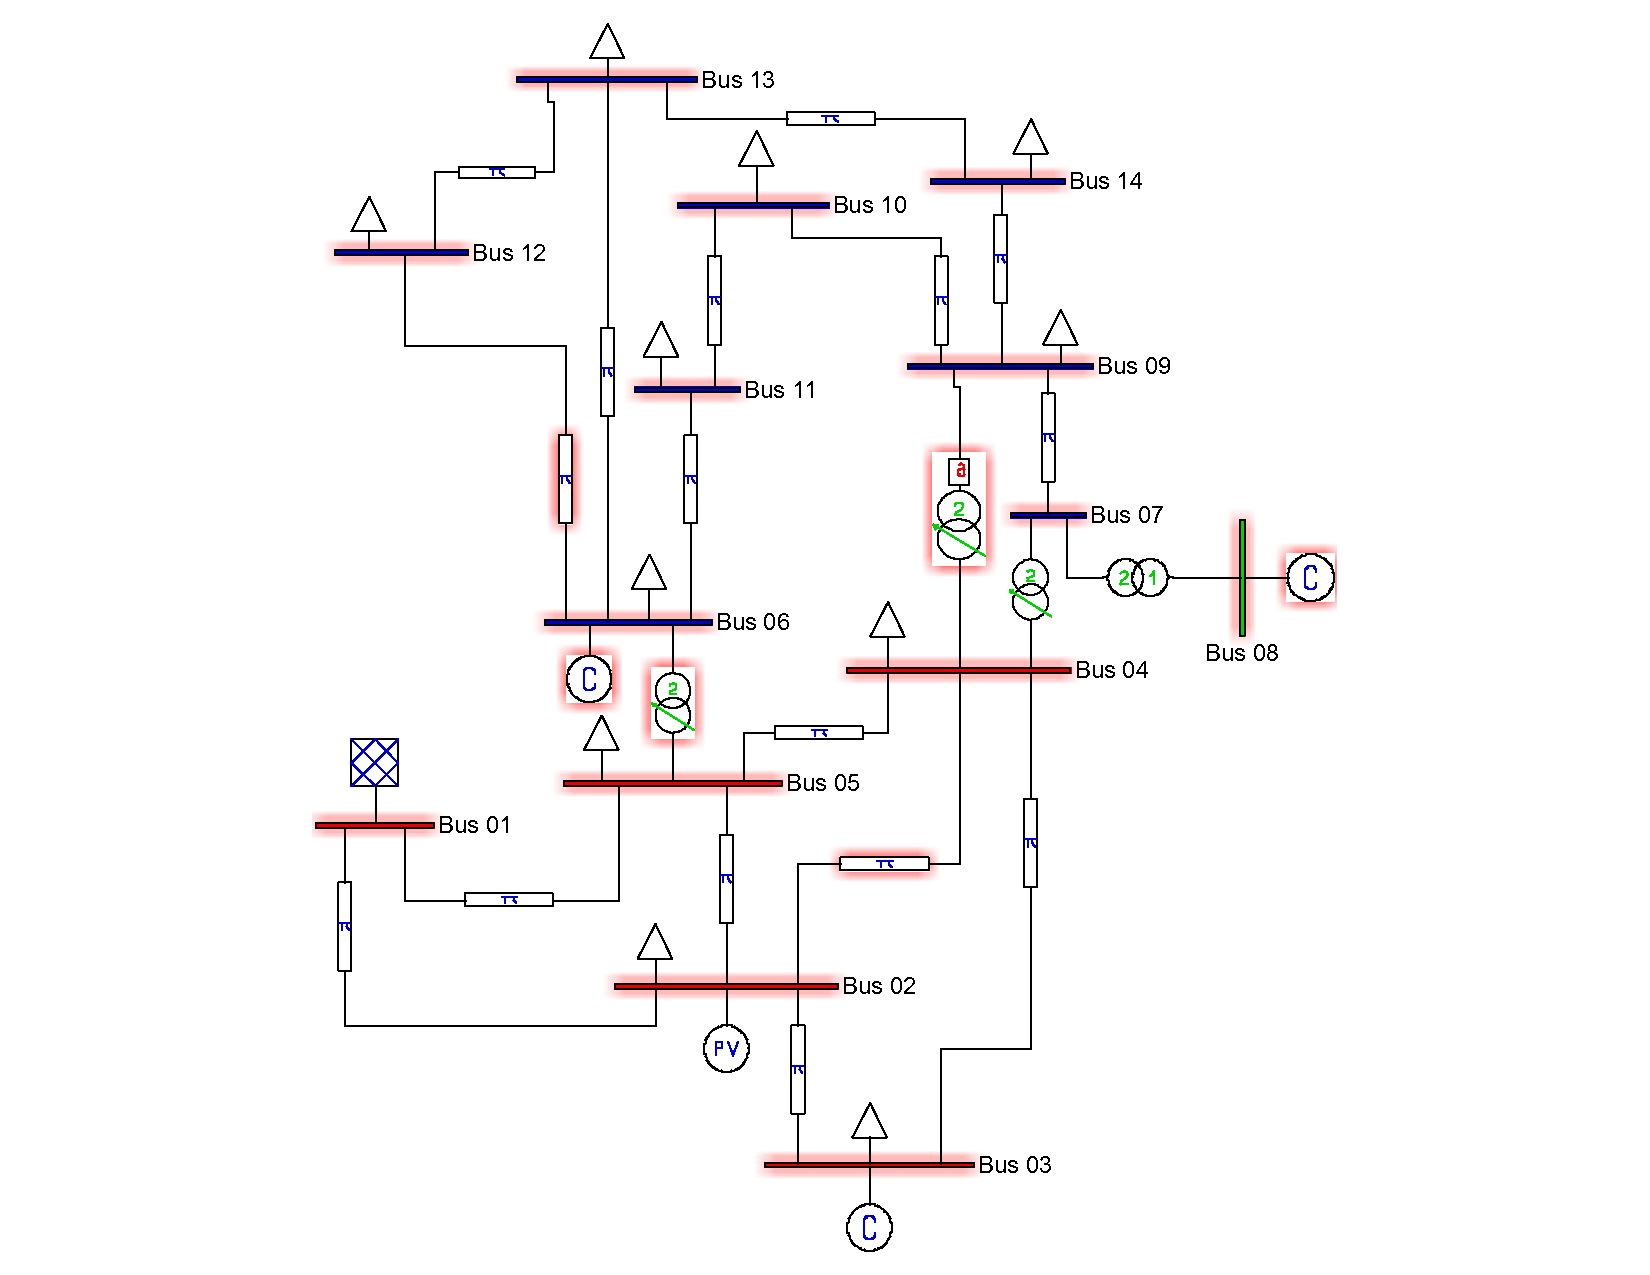
\includegraphics[height=13cm]{IEEE14.pdf}
  \caption{$IEEE14$电网拓扑原理图}
  \label{fig:fundement14}
\end{figure}

针对该拓扑,复杂网络的建模将其等效为一个无向图如图\ref{fig:model1},图中按照支路电气介数的大小等比例加粗了图的边,再根据图中的流程\ref{fig:nodeBetweenPro}最终计算得到各个节点的电气介数。电气介数计算的过程中,节点的电气介数直接受支路的电气介数影响。而支路的电气介数计算突出的是支路结构对能量分布的影响,能量分布越大的支路其电气介数也相应的越高。而$PangRank$的建模则将其等效为一个有向图如图\ref{fig:model2},再根据图\ref{fig:PRPro}最终计算得到各个节点的$PR$值。$PangRank$计算的过程中,突出的是拓扑的出入链的重要性。对于该模型,其迭代过程在能量转移矩阵的作用下完成,而入链累计度越高的点的$PangRank$越高。$PangRank$衡量了拓扑节点在能量转移中所起的作用。
\begin{figure}[H]
\begin{minipage}{0.48\textwidth}
  \centering
  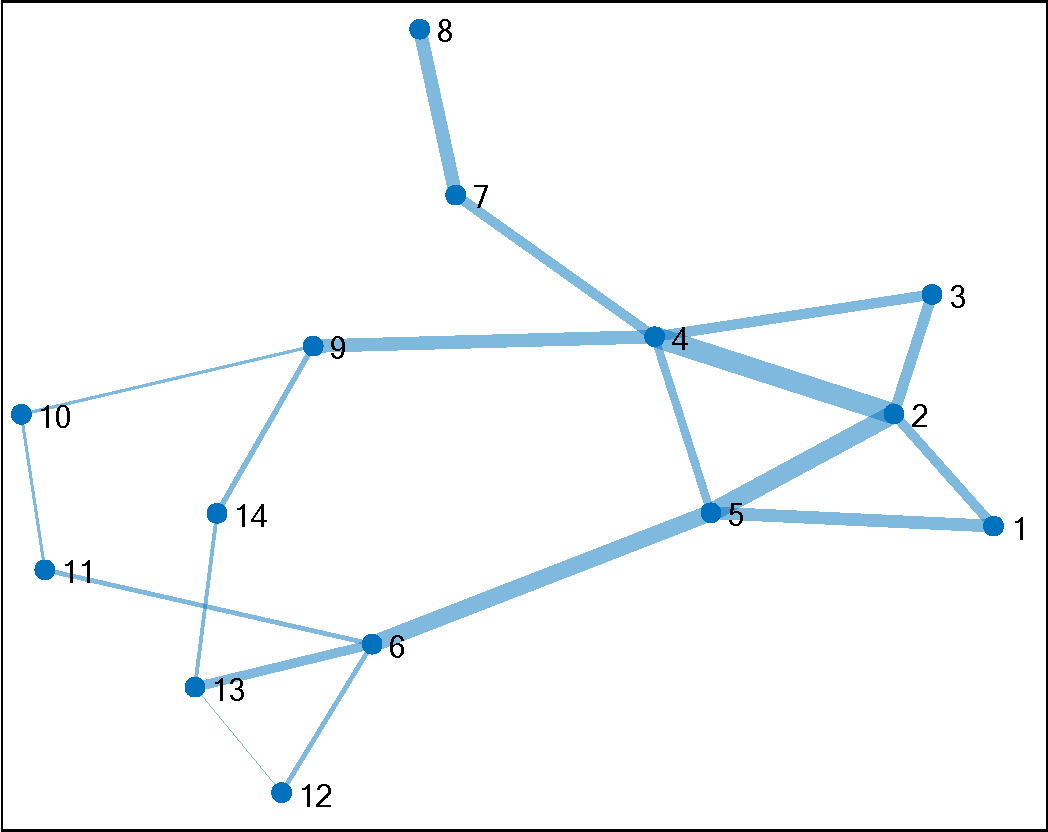
\includegraphics[height=5.8cm]{graph14.pdf}
  \caption{基于复杂网络的拓扑建模}
  \label{fig:model1}
\end{minipage}\hfill
\begin{minipage}{0.48\textwidth}
  \centering
  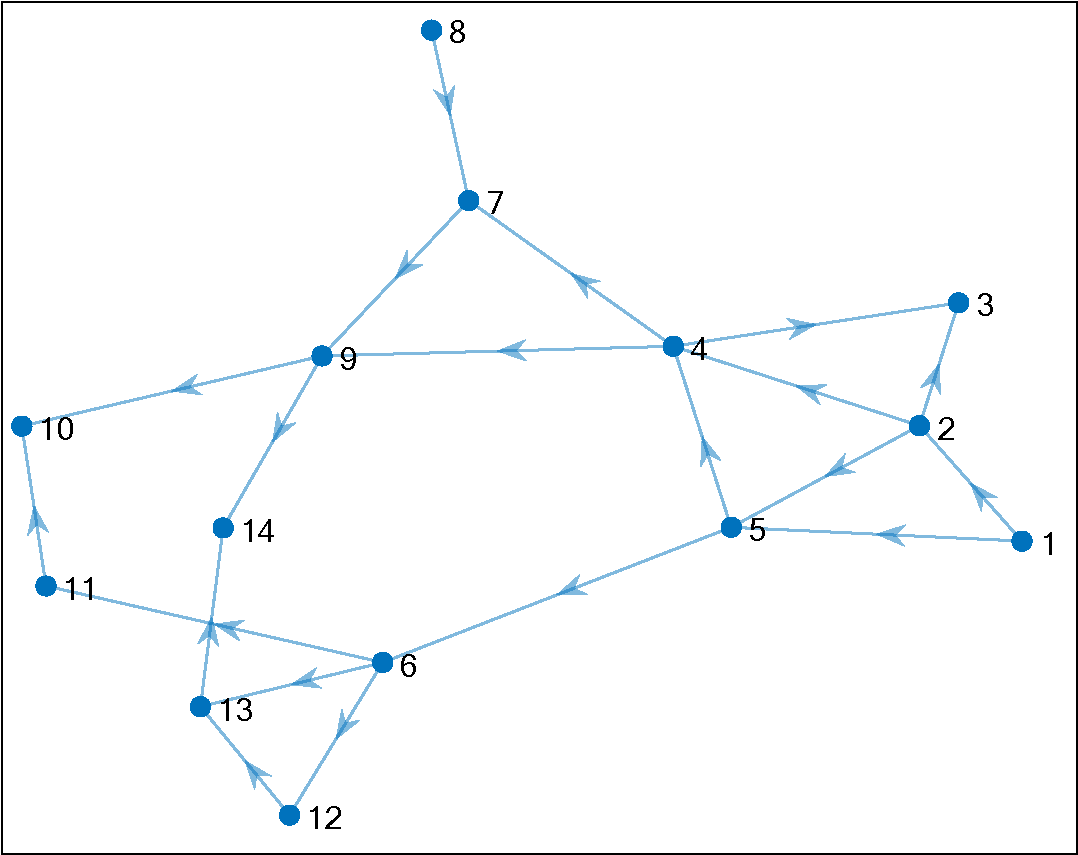
\includegraphics[height=5.8cm]{disgraph14.pdf}
  \caption{基于$PageRank$的拓扑建模}
  \label{fig:model2}
\end{minipage}
\end{figure}
电气介数与$PangRank$计算结果比较如图\ref{fig:compare_nodePR}。由于两个指标基于的拓扑模型不同,所以计算的结果相差较大。首先分析复杂网络的模型,从图中可以看出,支路的电气介数直接影响到了节点的电气介数,比如$2$、$4$、$5$节点由于与节点相连的支路比较重要而对拓扑具有较大的影响力。而支路的重要是因为$1$、$2$、$3$、$6$是系统中的发电节点,其功率传输分布因子较大,故而电电气阶数较大。而$4$、$5$处于发电和负荷的中间传输点,承担了较大的传输潮流的作用,因此相连的支路的电气介数都较大。$8$由于发电功率几乎为零且所连支路只有一条所以电气节数很小。而$12$、$11$、$10$负荷节点相连的支路都不是主要输送支路,功率传输因子小,所以电气节数较小。

反观$PangRank$的模型,该模型将每个节点的重要性赋予在该节点指向其他节点的出链上,因此,那些入链累计度高的节点重要性也高。比如$14$、$10$、$9$,这些节点均是负荷节点,能量最后传输给负荷,由于被潮流指向的累计的节点较多,即该节点的入链节点的入链节点数较多,因此重要性的权重被累计、叠加的程度较大。这种模型也符合现实,实际情况中,能量被输送、汇集到负荷节点,而负荷节点直接与用户相连,直接影响配电质量。因此,负荷节点在结构中的重要性非常高。在$PangRank$的模型中,由于发电节点是潮流起始点,$1$、$8$节点不仅是发电节点,而且是单向输出,没有其他入链,所以其$PR$值较小。

综上分析,电气介数与$PangRank$均对电力系统的结构特点进行了描述,均反映了各个节点在拓扑中的重要程度:前者从能量传输分布的角度对系统的拓扑进行了研究,后者从潮流累计分布的角度对拓扑进行了分析。因此,本文在第四章中将这两个指标进行了融合分析,作为结构脆弱性的综合评价指标。

\begin{figure}[H] % use float package if you want it here
  \centering
  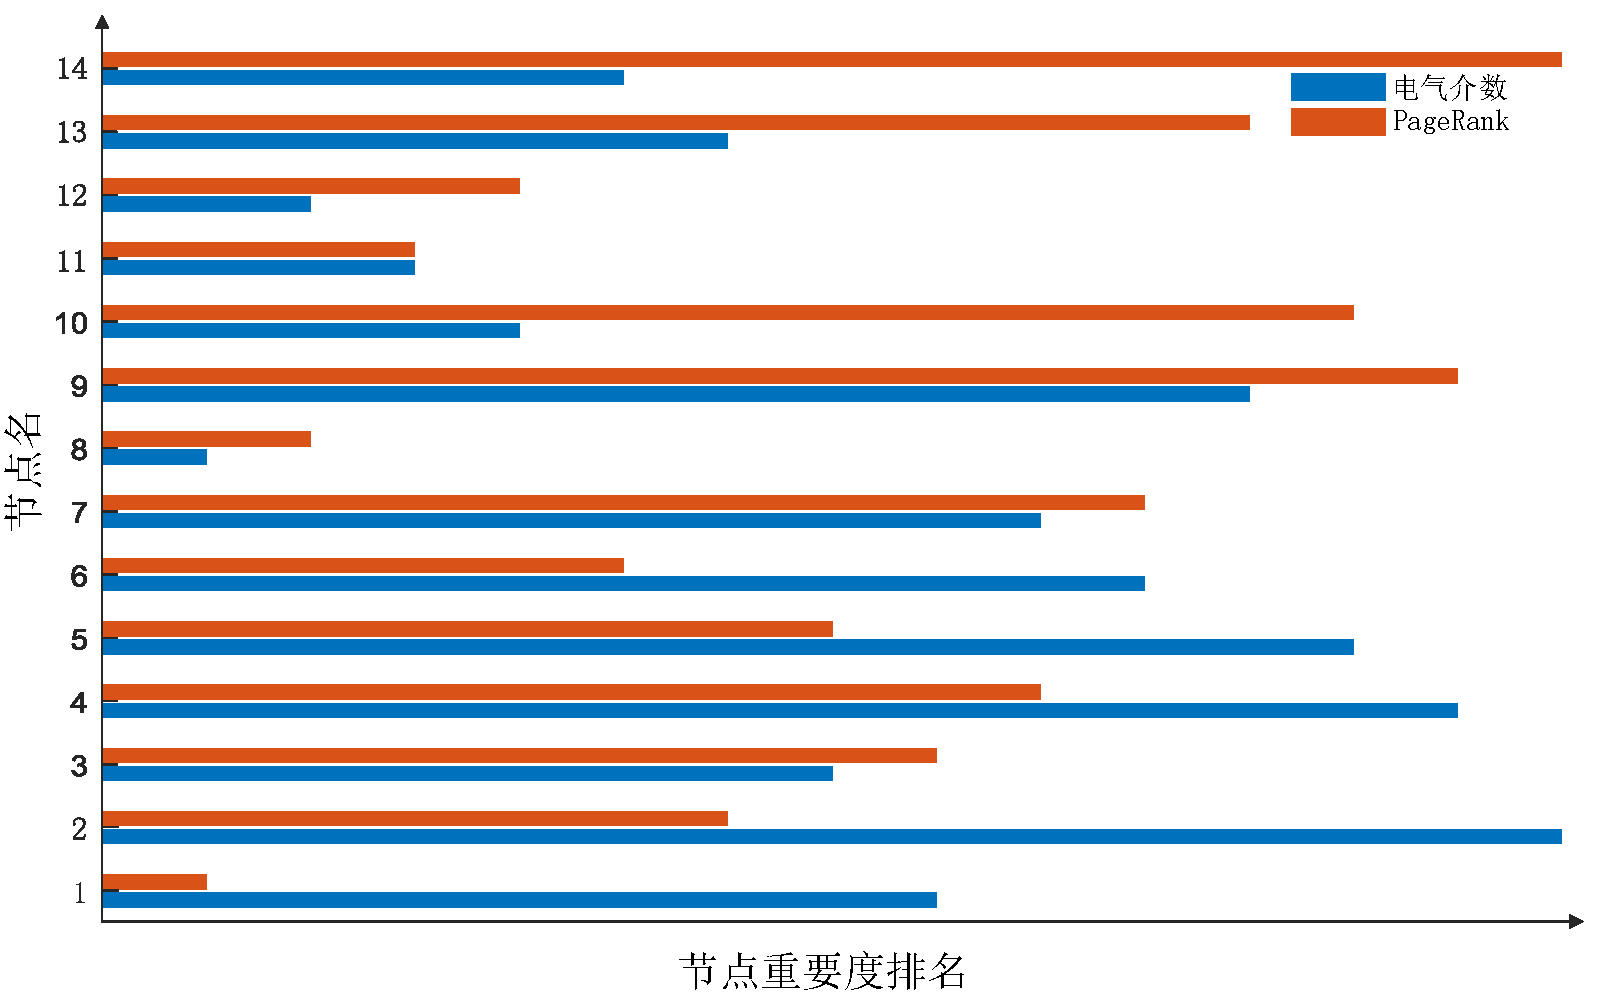
\includegraphics[height=8.7cm]{compare_nodePR.pdf}
  \caption{电气介数与$PangRank$计算结果比较图}
  \label{fig:compare_nodePR}
\end{figure}

\section{电力系统状态脆弱性研究}
\label{sec:status}



\subsection{电力系统状态脆弱性定义与数学描述}
\label{sec:vulneStaus}



\subsection{蒙特卡洛方法概述}
\label{sec:vulneStaus}






\subsection{负荷模型的建立}
\label{sec:vulneStaus}
结合状态三个指标的模型




\subsection{状态脆弱性分析方法及指标研究}
\label{sec:static}







\section{本章小结}
\label{sec:sum3}





